        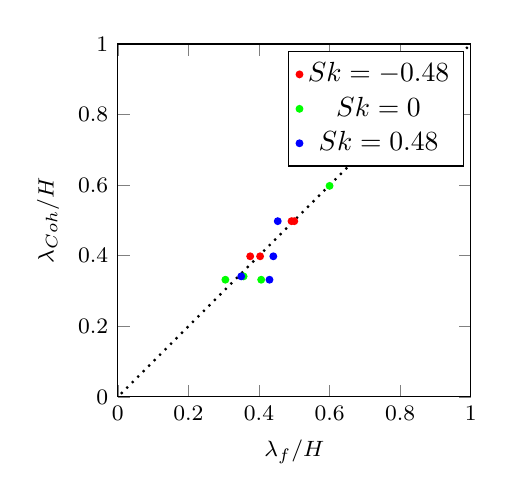
\begin{tikzpicture}[]
        \centering
        \begin{axis}[
            ylabel={$\lambda_{\text{Coh}}/H$},
			xlabel={$\lambda_f/H$},
			%xtick={-2,-1},
			%ytick={0,0.04,0.08},
			ymin=0,ymax=1,
			xmin=0,xmax=1,
            %ymin=0, ymax=0.16,
            width=.5\textwidth,
            height=.5\textwidth,
            label style={font=\footnotesize},
            tick label style={font=\footnotesize}
            ]
 \addplot [
           red,mark=*,only marks,thick, mark size=1pt
           ]
           coordinates{
		(0.4922,0.498)
            (0.5,0.498)
            (0.3750,0.3984)
            (0.4031,0.3984)
			};
			            \addlegendentry{$Sk=-0.48$}
\addplot [
            green,mark=*,only marks,thick, mark size=1pt
            ]
            coordinates{
            (0.3047,0.332)
            (0.4062,0.332)
            (0.3563,0.3415)
            (0.6,0.598)};
\addlegendentry{$Sk=0$}
               \addplot [
           blue,mark=*,only marks,thick, mark size=1pt
            ]
            coordinates{
            (0.4297,0.332)%P
           (0.4531,0.498)
            (0.3496,0.3415)
            (0.4406,0.3984)%
			};
			\addlegendentry{$Sk=0.48$}%
			\addplot [
            black,mark=square,thick,dotted,mark size=3pt
            ]
           coordinates{%
			(-0.1,-0.1)
			(1.1,1.1)
           };
        \end{axis}
        \end{tikzpicture}